\section{Related Work}\label{sec:related}

\subsection{Symbolic Score Following}
Classical real-time score following relies on symbolic scores such as MIDI or MusicXML. Online DTW \cite{dixon2005line} provides a straightforward baseline by incrementally matching audio frames to score events. Probabilistic state-space models offer richer temporal modeling: Cont \cite{cont2010coupled} introduced a coupled duration-focused architecture, while Arzt and Widmer \cite{arzt2010towards} addressed robustness under arbitrary performer deviations using multi-agent tracking. Particle-filter methods such as that of Korzeniowski et al.\ \cite{korzeniowski2013tracking} extended the probabilistic framework to handle tempo changes and rests. Jiang and Raphael \cite{jiang2020score} proposed a switching state-space model that tracks hidden tempo changes, improving alignment stability under expressive performance variation. Nakamura et al.\ \cite{nakamura2016real} modeled repeats and skips with an explicit transition structure. Their analysis further revealed that the majority of real-world score jumps are preceded by short silent breaks, an observation that motivates the jump recovery design in Section~\ref{subsec:jump}. More recently, Peter et al.\ \cite{peter2025pairing} combined real-time piano transcription with symbol-level tracking, achieving strong results by leveraging automatic music transcription as a front end. Matchmaker \cite{park2025matchmaker} provides a systematic evaluation framework for symbolic methods, though it does not cover image-based trackers.

\subsection{Image-Based Score Following}
Dorfer et al.\ \cite{dorfer2016towards} first showed that a multimodal convolutional neural network (CNN) can follow sheet music without symbolic input, classifying position into discrete staff-level buckets on small image crops. Reinforcement-learning formulations then framed the task as agent navigation over score strips \cite{dorfer2018rl,henkel2019score}. Henkel et al.\ \cite{henkel2020learning} moved to full-page processing via audio-conditioned U-Net segmentation, predicting a pixel mask whose center of mass gives the note position. CYOLO-SB \cite{henkel2021real} extended this to multi-resolution detection: three independent YOLO-style heads predict note, bar, and system bounding boxes from feature maps conditioned via Feature-wise Linear Modulation (FiLM)~\cite{perez2018film}. However, the three heads predict in parallel without cross-level constraints, predictions at each frame are decoded without temporal consistency constraints across frames, and no recovery mechanism exists for when tracking is lost.
\begin{figure*}[t]
\centering
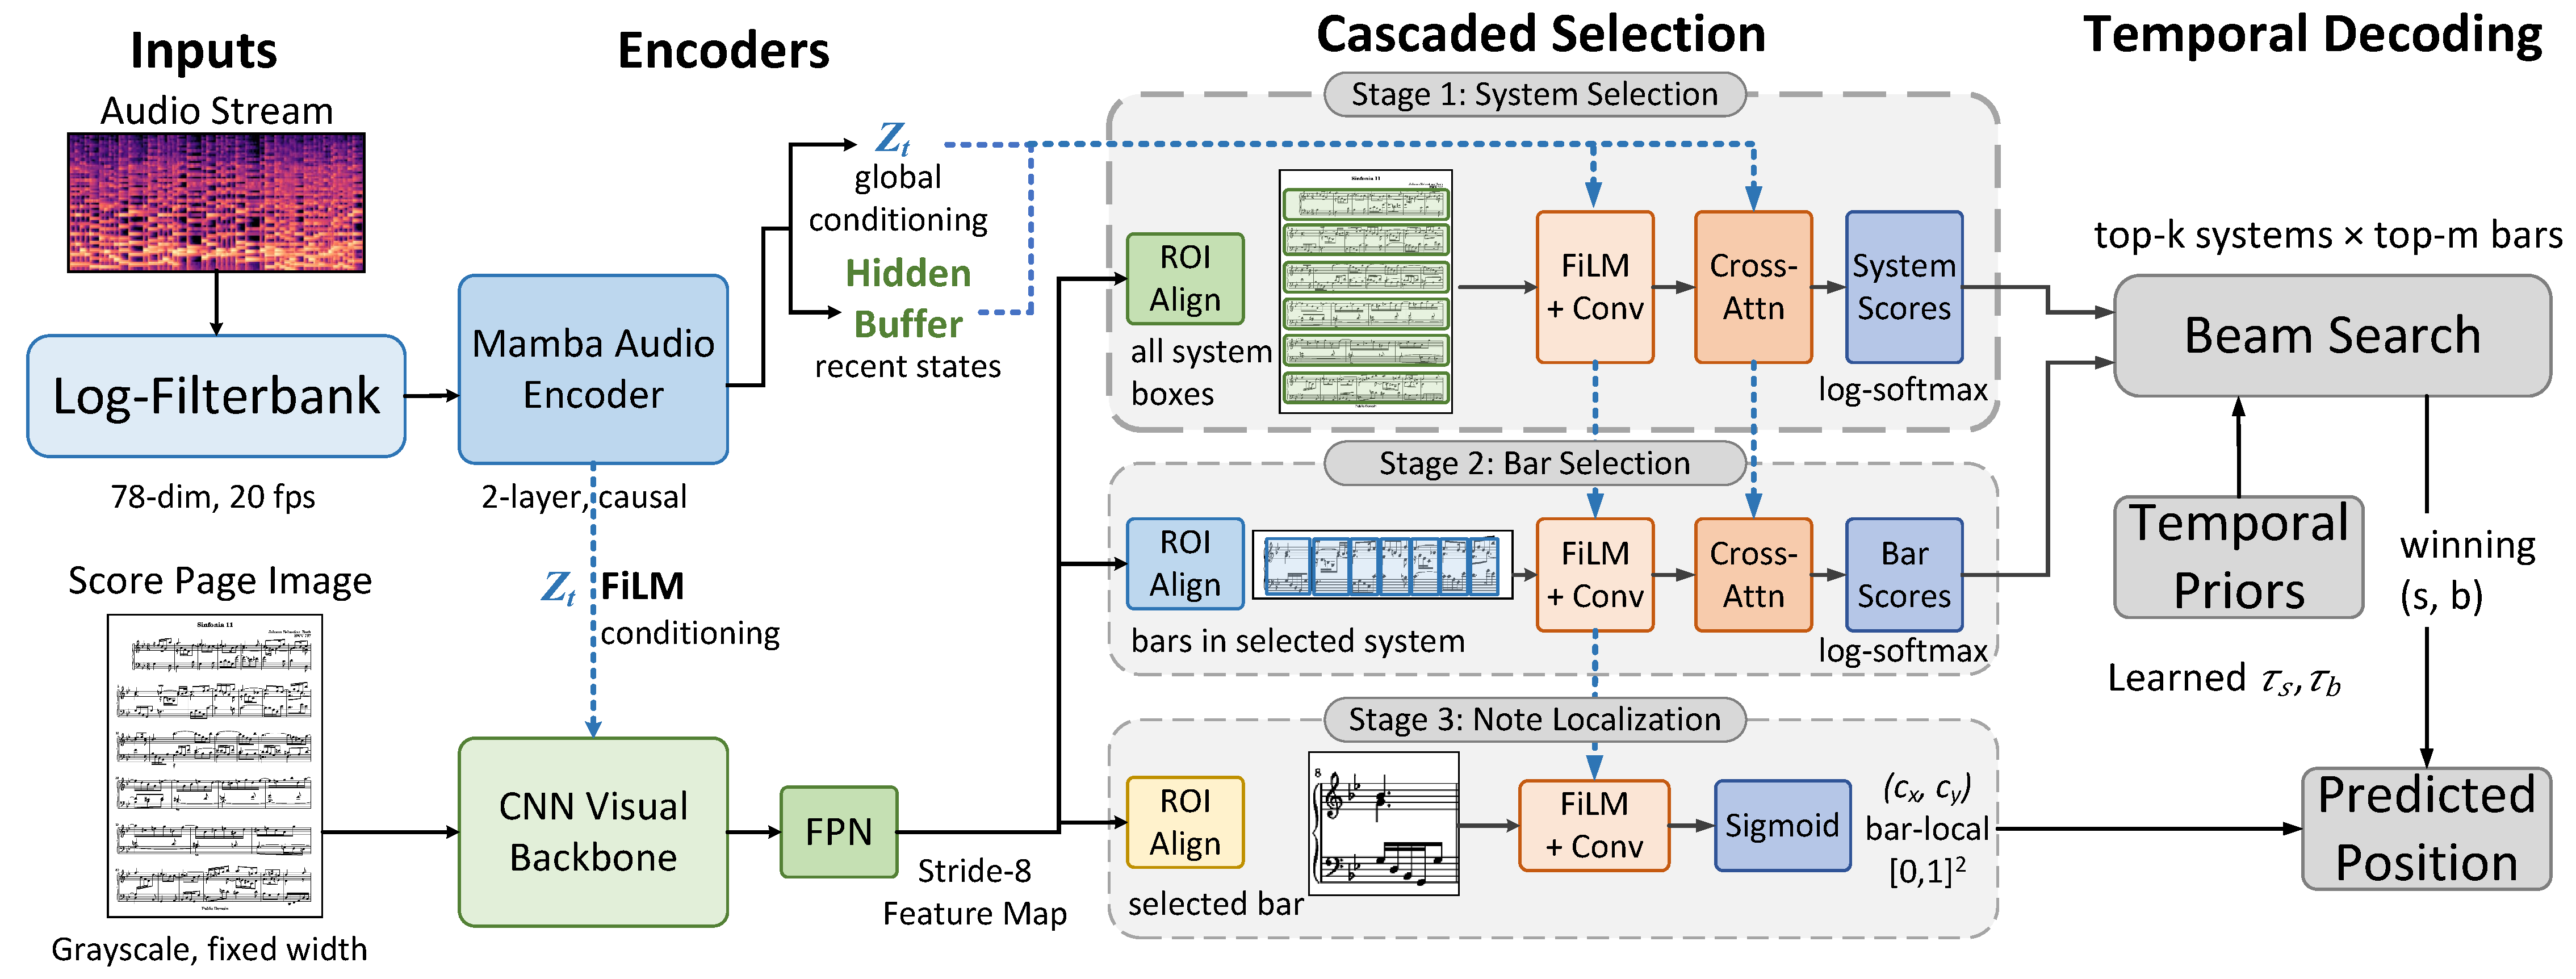
\includegraphics[width=\textwidth]{figures/overview.pdf}
\caption{Overview of the CODA architecture. A causal Mamba audio encoder and a shared CNN visual backbone feed into three cascaded stages: system selection, bar selection, and note localization. Beam search with learned temporal priors decodes the cascade over time.}
\label{fig:overview}
\end{figure*}

\subsection{Handling Repeats and Jumps}
Score discontinuities, including repeats, D.C., and coda jumps, pose a long-standing challenge for score following systems. In the symbolic domain, Nakamura et al.\ \cite{nakamura2016real} handle arbitrary repeats and skips through explicit state transitions. For offline audio-to-sheet-image synchronization, Shan and Tsai \cite{shan2020improved} proposed hierarchical DTW over learned audio and image features to handle repeats and jumps without requiring prior knowledge of jump locations. Morsi and Serra \cite{morsi2022bottlenecks} identified repeat handling as one of the key bottlenecks in audio-to-score alignment research. However, no existing real-time image-based score following method includes an explicit mechanism for recovering from score discontinuities during online tracking.

